\documentclass[11pt,a4paper]{article}

\usepackage[margin=2.5cm]{geometry}
\usepackage{amsmath}
\usepackage[T1]{fontenc}
\usepackage[utf8]{inputenc}
\usepackage{lmodern}
\usepackage{microtype}
\usepackage{booktabs}
\usepackage{tabularx}
\usepackage{longtable}
\usepackage{array}
\usepackage{enumitem}
\usepackage{xcolor}
\usepackage{hyperref}
\usepackage{caption}
\usepackage{float}
\usepackage{graphicx}

\definecolor{smublue}{RGB}{21,55,89}
\hypersetup{
  colorlinks=true,
  linkcolor=smublue,
  urlcolor=smublue,
  citecolor=smublue,
  pdftitle={From Forum Posts to Telco Actions},
  pdfauthor={Zixin}
}
\newcommand{\fitwidth}{\ifdim\width>\linewidth\linewidth\else\width\fi}
\setlength{\parindent}{0pt}
\setlength{\parskip}{0.55em}
\setlist{nosep}
\renewcommand{\arraystretch}{1.18}

\newcommand{\studentname}{Zixin [Surname]}
\newcommand{\studentid}{[Student ID]}
\newcommand{\programme}{[Programme / Course]}
\newcommand{\supervisorname}{[Professor's Name]}

\title{\textbf{From Forum Posts to Telco Actions}\\
\large An End-to-End Pipeline for Sentiment and Issue Analysis\\
of Singapore Telecommunications Discussions}
\author{\studentname\\\studentid\\\programme}
\date{September 2026}

\begin{document}

\begin{titlepage}
    \centering
    \vspace*{2cm}

    
\includegraphics[width=0.35\textwidth]{SMU_logo.png}\\[2cm]

    {\Large \textbf{School of Computing and Information Systems}}\\[0.5cm]
    {\Large \textbf{Singapore Management University}}\\[2cm]

    {\LARGE \textbf{Master of Science in Computing}}\\[1.5cm]

    {\Large \textbf{Capstone Project Report}}\\[2cm]

    {\Large \textbf{From Forum Posts to Telco Actions:\\ An End-to-End Pipeline for Sentiment and Issue Analysis\\ of Singapore Telecommunications Discussions}}\\[2cm]

    \vfill

    \begin{tabular}{ll}
        \textbf{Student Name:} & Liao Zixin \\
        \textbf{Track:} & Data Science \& Data Analytics \\
        \textbf{Supervisor:} & Kyong Jin SHIM \\
        \textbf{Project Duration:} & Dec 2025 -- Oct 2026 \\
        \textbf{Date:} & October 16th, 2026 \\
    \end{tabular}

    \vfill
\end{titlepage}

\begin{abstract}
Singapore telecommunications operators receive continuous, unsolicited customer feedback through online forums, but the volume, informality and platform-specific language make manual monitoring difficult. This project develops an end-to-end pipeline that collects forum discussions, normalises heterogeneous records, identifies telecommunications brands, assigns sentiment and issue labels, and presents findings through a static HTML dashboard. The analysis corpus combines Reddit and HardwareZone (HWZ) posts up to 26~September~2026: after removing repeated copies and off-topic threads, 9,162 unique posts in 349 telco threads remain. GPT-4o-mini labels 44\% of them not happy and 19\% happy (42\% and 18\% with threads weighted equally), whereas VADER on the same posts reports 28\% and 46\%. Network quality is the largest issue theme (37--41\% of posts), followed by mobile plans (13--14\%) and pricing (7--8\%). Reddit and HWZ differ mainly in topic rather than tone, and no brand stands out beyond small, weighting-sensitive differences. One event shows why that care is needed: 45 outage threads, led by the March 2026 Singtel outage, hold 12\% of posts, are 71\% not happy against 40\% elsewhere, and sit almost entirely on Reddit, which creates most of the apparent Reddit--HWZ gap.

The system combines deterministic brand matching, VADER sentiment, a keyword issue taxonomy and OpenAI chat-completions classification. Independent human labels on a blinded 400-post representative sample covering the whole collection period (392 telco-relevant posts) show that \textbf{gpt-4o-mini-2024-07-18} improves sentiment over VADER (macro F1 0.641 versus 0.380; accuracy 66\% versus 39\%). \textbf{gpt-4o-2024-08-06} is no better on sentiment (macro F1 0.611) and only ties keyword issue rules when it labels every post (macro F1 0.585 versus 0.590). A hybrid that keeps rule labels and applies GPT-4o only to unresolved \texttt{general\_discussion} rows raises issue macro F1 to \textbf{0.639}, and was applied to all 12,497 unresolved corpus rows (about 41 minutes, estimated \textbf{\$4.80}). On a held-out 100-post challenge set of harder posts, the sentiment result holds (GPT-4o-mini 0.773 versus VADER 0.491), but the hybrid's gain over rules is not significant (0.509 versus 0.499) and GPT-4o labelling every post scores best (0.596), so no single issue method wins on both sets. Two human annotators agree only fairly on typical posts ($\kappa=0.39$), mostly over whether a bare failure report is a complaint; without that one pattern agreement reaches 0.57, and GPT-4o-mini agrees with each annotator about as well as they agree with each other. GPT-4o-mini sentiment on all 9,162 posts cost about \$0.28, and a repeated run reproduced 292 of 295 gold-set labels. The operational recommendation is therefore LLM sentiment (mini is sufficient), keyword rules plus a targeted GPT-4o pass for issues, and human review of alerts. The business analysis indicates that operators should prioritise incident communication during outages, comparable plan terms such as fair-use limits and add-on charges, and equipment and app friction, with billing and customer-service aftercare planned for incidents; roaming and porting are small in this corpus. The principal contribution is a reproducible analytics workflow that converts noisy forum data into decision-oriented signals while making its evidential limits explicit.
\end{abstract}

\vfill
\begin{center}
\small\textit{Keywords:} telecommunications, social listening, sentiment analysis, issue extraction, VADER, large language model, dashboard
\end{center}
\newpage

\tableofcontents
\newpage

\section{Introduction}

\subsection{Background, objectives and research questions}

Mobile customers discuss price plans, coverage, roaming, porting and service failures in public online communities. These discussions can reveal emerging pain points earlier and in more detail than periodic surveys, which is why opinion mining from online text has become a standard source of customer insight \cite{pang2008opinion}. They are also difficult to analyse reliably: posts contain Singlish, abbreviations, sarcasm, quoted text, multiple brands and off-topic uses of ambiguous brand names such as ``Eight'' or ``M1'' \cite{liu2012sentiment}.

This project asks how a telecommunications operator can convert such unstructured discussion into a repeatable source of customer insight. The objective is not to infer population-level satisfaction or replace operational metrics. Instead, the pipeline is designed as an early-warning and exploratory decision-support system that helps analysts locate themes, compare discussion contexts and inspect representative records. To do this, the project collects relevant discussions from multiple online platforms, cleans and standardises the heterogeneous post and comment records, detects the mentioned operators and classifies sentiment and service issues, compares lightweight baselines with more context-aware model options, and translates the results into actionable recommendations through a dashboard.

Four research questions guide the work. RQ1 asks which sentiment and issue themes appear most frequently in the collected Singapore telco discussions. RQ2 asks how discussion patterns differ between Reddit and HWZ, and across telco brands. RQ3 asks what additional value a context-aware model provides over VADER sentiment and keyword-based issue rules. RQ4 asks how the extracted signals can support concrete decisions by telco operators.

\subsection{Scope and claimed contribution}

The repository implements collection modules for HWZ and Reddit. It includes preprocessing, brand detection, sentiment labelling, issue extraction, evaluation scripts and a static HTML dashboard. The report only claims findings supported by persisted repository outputs. GPT-4o-mini and GPT-4o are evaluated on human labels for both the representative and challenge sets, and GPT-4o is used on unresolved corpus issues. The findings and dashboard use GPT-4o-mini sentiment and hybrid issue labels on the 9,162-post corpus.

\section{Data and Pipeline}

\subsection{Data sources}

The corpus covers Reddit posts from Singapore-focused communities, matched on telco and mobile-plan keywords, and HWZ posts from relevant XenForo threads, up to 26~September~2026. Reddit posts up to 9~April~2026 came from the public JSON interface; because Reddit then blocked unauthenticated access and gated new API applications, later Reddit posts and comments (including replies) came from the Arctic Shift research archive \cite{arcticshift}, filtered with the same strict brand rule. A page-counter bug meant early HWZ scrapes read only the first page of each thread; after the fix, the newest pages of each telco thread were collected as well. The scrapers preserve thread titles, post or comment text, timestamps, source identifiers and available engagement metadata.

\begin{table}[H]
\centering
\caption{Persisted analytical datasets}
\label{tab:data}
\begin{tabularx}{\textwidth}{@{}p{0.34\textwidth}rX@{}}
\toprule
\textbf{Dataset} & \textbf{Rows} & \textbf{Role} \\
\midrule
\texttt{issues\_\allowbreak{}posts\_\allowbreak{}labeled\_\allowbreak{}\ldots\_\allowbreak{}gpt4o\_\allowbreak{}hybrid.csv} & 24,690 & All scraped rows after preprocessing, with brand, VADER and issue labels (rules plus GPT-4o on 12,497 unresolved rows) \\
\texttt{corpus\_\allowbreak{}posts.csv} & 9,162 & Clean corpus: unique posts in 349 telco threads \\
\texttt{corpus\_\allowbreak{}posts\_\allowbreak{}mini\_\allowbreak{}sentiment.csv} & 9,162 & Clean corpus with GPT-4o-mini sentiment; findings and dashboard input \\
\texttt{gold\_\allowbreak{}labels.csv} & 500 & Annotator~A's blind gold sheets in one file: the representative set (400 posts in two date-based samples, 392 telco-relevant; headline metrics) and the challenge set (100 harder posts; held out) \\
\texttt{merged\_\allowbreak{}gold\_\allowbreak{}scores.json} & 392 & Every method scored on the representative set: macro F1, per-class metrics, bootstrap intervals, $\kappa$ \\
\texttt{llm\_\allowbreak{}comparison\_\allowbreak{}representative/\allowbreak{}} & 295 & GPT-4o-mini vs VADER/rules predictions, metrics, tokens and cost \\
\texttt{llm\_\allowbreak{}comparison\_\allowbreak{}representative\_\allowbreak{}gpt4o/\allowbreak{}} & 295 & GPT-4o vs VADER/rules on the same gold labels \\
\texttt{llm\_\allowbreak{}comparison\_\allowbreak{}representative\_\allowbreak{}gpt4o\_\allowbreak{}hybrid/\allowbreak{}} & 295 & Rules, then GPT-4o only where rules output \texttt{general\_\allowbreak{}discussion} \\
\texttt{llm\_\allowbreak{}comparison\_\allowbreak{}challenge\_\allowbreak{}gpt4o/\allowbreak{}} & 100 & GPT-4o vs VADER/rules on the challenge set; hybrid scored from it \\
\texttt{robustness\_\allowbreak{}summary.json} & --- & Bootstrap intervals, run-to-run stability, annotator agreement, corpus checks \\
\bottomrule
\end{tabularx}
\end{table}

The scraped rows are not independent posts. The 24,690 labelled rows hold 11,643 unique posts, because successive scrape rounds saved the same comments again; in one ten-round scrape, rounds 2--9 added no new posts. Ninety-six of 445 threads were off-topic and matched a keyword by accident, such as a 248-post thread on what feels cheaper in Singapore and a 98-post insurance lawsuit thread. \texttt{processing/build\_clean\_corpus.py} keeps one row per post ID (Reddit comment or post ID; HWZ thread URL and timestamp), so identical text from different users stays separate, and drops a thread unless at least 20\% of its posts name a telco or its title is telco-related. The result is 9,162 posts in 349 threads (5,711 Reddit, 3,451 HWZ).

\subsection{Preprocessing}

The preprocessing module maps platform-specific fields to a common schema, removes empty, placeholder and very short records, and can optionally retain English-language records using language detection. The common schema includes \texttt{source}, \texttt{thread\_title}, \texttt{post\_text}, timestamp fields and identifiers. Normalisation allows downstream modules to process different platforms without source-specific model code.

The current workflow retains post text that may include informal spelling, emoji and HTML entities because these features can carry sentiment. This is useful for analysis but also creates modelling challenges. The dashboard therefore presents aggregate indicators and traceable examples rather than treating model output as verified customer facts.

\subsection{End-to-end architecture}

Figure~\ref{fig:pipeline} shows the implemented sequence. Seven steps run from scraping to the dashboard. Preprocessing and issue extraction are expanded to show what each one does, and a separate branch scores the model outputs against the human gold labels. The gold labels do not feed back into the data; they only check the sentiment and issue labels.

\begin{figure}[htbp]
\centering
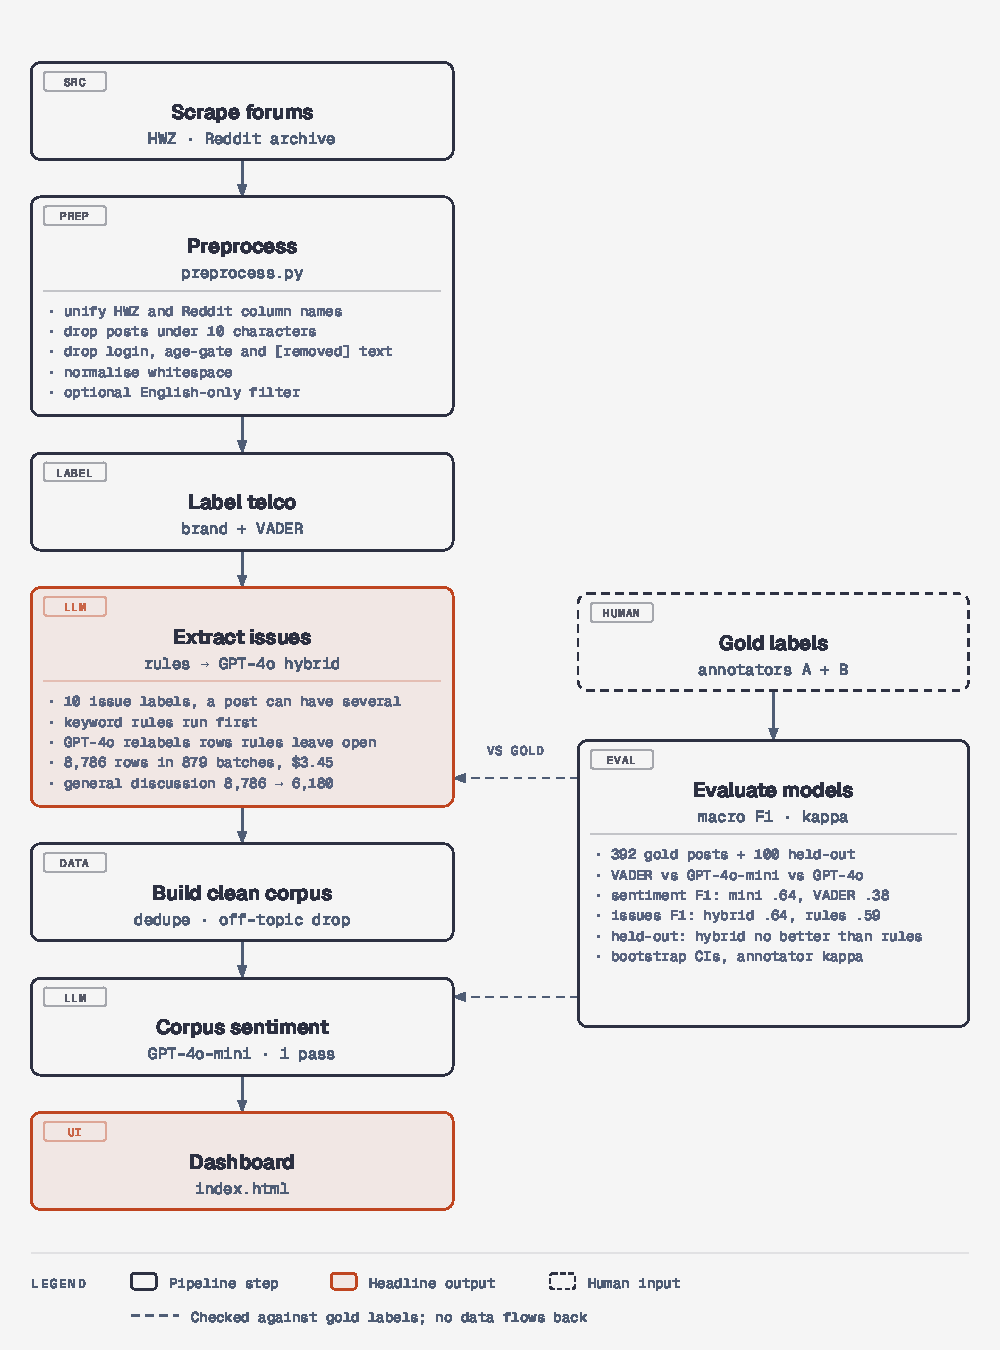
\includegraphics[width=0.88\textwidth]{pipeline.pdf}
\caption{End-to-end pipeline. Boxes in the left column are the data steps. The right column is the evaluation branch: dashed arrows mark checks against human gold labels, not data flow. Accent colour marks the hybrid issue labels and the dashboard, the two headline outputs.}
\label{fig:pipeline}
\end{figure}

The static dashboard generator is deliberately lightweight and produces a standalone HTML report that opens in any browser without a server.

\section{Analytical Methods}

\subsection{Telco detection}

Brand mentions are identified by regular expressions over the concatenated thread title and post text. The tracked labels include Singtel, StarHub, M1, SIMBA, Giga, Eight, Zym and redONE, with additional MVNO keywords used by the dashboard. Multiple brands can be assigned to one record. This design is transparent and inexpensive, but ambiguous names and thread-level context can create false positives. For example, a post containing the ordinary word ``eight'' may be incorrectly associated with the Eight brand unless the surrounding context is considered.

\subsection{Sentiment baseline: VADER}

VADER is a lexicon- and rule-based sentiment method designed for social-media text \cite{hutto2014vader}. For each post, the pipeline obtains a compound score and maps it to:

\begin{equation}
\text{label}(s)=
\begin{cases}
\text{happy}, & s \geq 0.05,\\
\text{not\_happy}, & s \leq -0.05,\\
\text{neutral}, & \text{otherwise}.
\end{cases}
\end{equation}

VADER is a suitable operational baseline because it runs locally, is deterministic and requires no paid API. Its limitation is contextual understanding. It can misread sarcasm, negation over long passages, mixed opinions, quoted complaints and the difference between sentiment towards a telco and sentiment towards another topic in the same thread.

\subsection{LLM sentiment}

The labelling module implements LLM sentiment through an OpenAI-compatible chat-completions interface. Its configured default is \textbf{GPT-4o-mini} \cite{openai2024gpt4o}. Formal comparison uses the snapshots returned by the API, \textbf{gpt-4o-mini-2024-07-18} and \textbf{gpt-4o-2024-08-06}, with temperature 0 and JSON object responses in batches of ten posts. The corpus was labelled with the same prompt, batching and settings through \texttt{models/corpus\_llm\_sentiment.py}; the checkpoint is keyed by post ID, so posts already labelled in an earlier run were not sent again. Labelling all 9,162 posts cost about \$0.28.

\subsection{Issue taxonomy and rationale}

The issue taxonomy contains ten business-facing categories. These labels were selected because they separate product, network, service, billing, digital-channel and device decisions while retaining a general-discussion fallback:

\begin{table}[H]
\centering
\caption{Issue taxonomy and business rationale}
\label{tab:taxonomy}
\begin{tabularx}{\textwidth}{@{}p{0.19\textwidth}p{0.35\textwidth}X@{}}
\toprule
\textbf{Label} & \textbf{Typical evidence} & \textbf{Action owner / decision} \\
\midrule
Network Quality & coverage, signal, 4G/5G, speed, latency, outage & Network teams: local investigation, capacity and coverage communication \\
Pricing \& Promotions & price, promotion, discount, deal, cashback & Commercial teams: price communication and promotion fulfilment \\
Mobile Plans & SIM-only allowances, contract terms, minutes, SMS & Product teams: plan design and feature comparison \\
Roaming & overseas data, IDD, APAC, international use & Roaming teams: bundles, activation and destination guidance \\
Porting & port-in/out, number transfer, switching & Operations: mobile-number-portability workflow and exception handling \\
Customer Service & support, hotline, agent, complaint, escalation & Service operations: contact journeys and case resolution \\
Billing \& Payment & bills, charges, refunds, invoices, GIRO & Billing teams: charging controls and payment resolution \\
App \& Account & app, login, password, OTP, verification, portal & Digital teams: self-service access and account management \\
Devices & phones, eSIM/SIM, routers, ONR/ONT, equipment & Device and technical teams: compatibility and equipment support \\
General Discussion & telco news, opinions, no specific issue & Analysts: monitor broad conversation and review taxonomy coverage \\
\bottomrule
\end{tabularx}
\end{table}

The categories remain compact enough to route to owners while separating previously conflated topics such as plan design from promotions, billing from customer service, and app access from device problems. Multi-label output permits a post to mention, for example, both pricing and roaming. The rule-based classifier assigns labels when predefined regular expressions match and otherwise assigns \texttt{general\_discussion}. GPT-4o was then applied only to those unresolved rows. On the representative gold set that hybrid beats both keyword-only and all-row LLM tagging, so it was run on the 8,786 unresolved corpus rows. Section~\ref{sec:challenge} tests it on held-out posts.

\section{Evaluation Design and Evidence}

\subsection{Required metrics}

For a three-class sentiment task, overall accuracy alone can hide poor performance on minority classes. The evaluation module therefore calculates a confusion matrix and per-class precision, recall and F1, together with macro F1. For issue extraction, the appropriate measures are per-class precision, recall and F1 under a multi-label protocol, plus micro and macro averages.

Model comparison uses the same independently annotated records. Runtime is measured on the same machine, and the API run records input tokens, output tokens, retries, the exact returned model identifier and estimated cost from the provider list prices supplied at run time.

\subsection{Independent annotation}

A blinded evaluation package was generated without VADER or LLM columns: each sheet shows only the thread title and the post. Annotator~A labelled two gold sets, drawn with the same rules (posts naming a telco, one copy of each text, at most five posts per thread in each sample):

\begin{itemize}
  \item a 400-post representative set, drawn in two samples so that it covers the whole collection period: 300 posts collected up to 9~April~2026 (214 Reddit, 86 HWZ) and 100 posts published from 10~April to 26~September~2026 (56 Reddit, 44 HWZ). Of these, 392 are telco-relevant and carry the headline metrics;
  \item a 100-post challenge set reserved for harder cases (negation, sarcasm or Singlish cues, mixed brands, weak VADER scores, long posts), drawn from threads not in the first representative sample.
\end{itemize}

The two sets share no posts. Eight later representative posts come from three long HWZ threads that also contribute challenge posts, and seven threads contribute six to eight representative posts across the two samples. Challenge metrics are reported separately and never pooled with the representative set. Two misspelt issue labels in the later sheet were normalised at scoring time, and four relevant posts with no issue label are left out of the issue scores, so issue metrics use 388 posts. All representative scores come from \texttt{models/score\_merged\_gold.py}, which writes \texttt{merged\_gold\_scores.json} and makes no API calls.

\subsection{Human agreement}
\label{sec:agreement}

A second annotator labelled a 100-post overlap (60 representative, 40 challenge; \texttt{double\_annotation\_\allowbreak annotator\_b\_\allowbreak filled2.csv}). Sentiment agreement is fair on typical posts and moderate on hard ones (bands from \cite{landis1977kappa}): 62\% raw agreement and Cohen's $\kappa=0.39$ \cite{cohen1960kappa} on the representative overlap ($n=58$), and 73\% with $\kappa=0.59$ on the challenge overlap ($n=40$). On the challenge overlap, 9 of 40 rows match Annotator~A on every field and no notes are identical.

The low agreement has one main cause. Most disagreements share a single pattern: posts Annotator~A labelled \texttt{not\_happy} that Annotator~B labelled \texttt{neutral} (9 of 22 disagreements on the representative overlap, 8 of 11 on the challenge overlap). They are typically bare failure reports, questions about compensation and troubleshooting advice. The annotation guide originally listed ``service failure'' under \texttt{not\_happy} and ``factual statement'' under \texttt{neutral} without saying which takes precedence; it now states that a first-hand failure report is \texttt{not\_happy}. Annotator~B's relabelling applies that rule, while Annotator~A's labels predate it. Table~\ref{tab:agreement} shows how much this one pattern matters, and how GPT-4o-mini compares with the two humans on the same posts.

\begin{table}[H]
\centering
\caption{Cohen's $\kappa$ for sentiment on the annotator-B overlap (posts with all three labels)}
\label{tab:agreement}
\begin{tabular}{lrr}
\toprule
\textbf{Pair} & \textbf{Representative ($n=57$)} & \textbf{Challenge ($n=40$)} \\
\midrule
Annotator~A vs Annotator~B & 0.37 & 0.59 \\
A vs B, disputed pattern removed & 0.57 & 0.86 \\
GPT-4o-mini vs Annotator~A & 0.33 & 0.66 \\
GPT-4o-mini vs Annotator~B & 0.52 & 0.54 \\
\bottomrule
\end{tabular}
\end{table}

Three points follow. First, removing the one disputed pattern lifts agreement to 0.57 and 0.86, so the low $\kappa$ reflects one ambiguous rule rather than general disagreement about tone. Second, GPT-4o-mini agrees with each annotator about as well as the two annotators agree with each other, so on this evidence the model sits within the range of human judgement. Third, the human ceiling bounds every score in this chapter: no method can be expected to score near 1.0 against one annotator, and small differences between methods should be read through their bootstrap intervals. The sentiment gap between GPT-4o-mini and VADER (Table~\ref{tab:headlinemetrics}) is far larger than this noise. Issue agreement is weakest on small labels (Devices $\kappa=0.16$, App \& Account 0.17, Customer Service 0.28, against Network Quality 0.79). Adjudicating the disagreements and relabelling Annotator~A's overlap rows under the new rule is the next step for the benchmark (Section~\ref{sec:future}).

\subsection{Headline comparison (representative, $n=392$)}

Table~\ref{tab:headlinemetrics} compares GPT-4o-mini and GPT-4o with the local baselines on the 392 representative posts (388 for issues). Sentiment support is 82 happy, 186 not happy and 124 neutral. GPT-4o-mini sentiment comes from the evaluation run for the 300-post sample and from the production corpus labels for the later 100, with the same prompt and settings. GPT-4o was run on the 388 posts that carry issue labels, so its rows and every comparison with it use those posts. The hybrid issue row keeps keyword labels except where rules output only \texttt{general\_discussion}, then substitutes GPT-4o's issue list.

\begin{table}[H]
\centering
\small
\caption{Representative-set comparison against Annotator~A labels}
\label{tab:headlinemetrics}
\resizebox{\fitwidth}{!}{%
\begin{tabular}{lrrrr}
\toprule
\textbf{Task / method} & \textbf{Accuracy} & \textbf{Macro F1} & \textbf{Micro F1} & \textbf{Exact match} \\
\midrule
Sentiment: VADER & 0.385 & 0.380 & --- & --- \\
Sentiment: GPT-4o-mini & 0.661 & \textbf{0.641} & --- & --- \\
Sentiment: GPT-4o & 0.649 & 0.611 & --- & --- \\
Issues: keyword rules & --- & 0.590 & 0.606 & 0.335 \\
Issues: GPT-4o-mini & --- & 0.498 & 0.515 & 0.302 \\
Issues: GPT-4o (all rows) & --- & 0.585 & 0.628 & 0.353 \\
Issues: GPT-4o hybrid (unresolved only) & --- & \textbf{0.639} & \textbf{0.674} & \textbf{0.387} \\
\bottomrule
\end{tabular}%
}
\end{table}

GPT-4o-mini is at least as good as GPT-4o on sentiment at about one-seventeenth of the cost. No all-row LLM beats keyword rules on issues: GPT-4o closes most of the mini gap (0.498 to 0.585) but only ties rules (0.590). The unresolved-only hybrid is the only issue method that beats rules, because it keeps Devices and other keyword-heavy labels and spends the model only on the 129 gold posts that rules could not classify.

Paired bootstrap intervals (2,000 resamples of the posts, fixed seed \cite{efron1993bootstrap}) separate real gains from ties. GPT-4o-mini beats VADER on sentiment by 0.261 macro F1 (95\% CI 0.197 to 0.324). GPT-4o-mini and GPT-4o are tied (difference 0.029, CI $-0.020$ to 0.080). On issues, rules beat all-row GPT-4o-mini (0.092, CI 0.037 to 0.146) and tie all-row GPT-4o (GPT-4o minus rules $-0.005$, CI $-0.053$ to 0.042), while the hybrid beats both rules (0.049, CI 0.024 to 0.074) and all-row GPT-4o (0.054, CI 0.016 to 0.092). A second GPT-4o-mini run on the 295 relevant posts of the first sample reproduced 292 of them (run-to-run $\kappa=0.98$; macro F1 0.631 and 0.627), so the model's own run-to-run variation is far smaller than these differences.

\begin{table}[H]
\centering
\caption{VADER sentiment confusion matrix, representative set (rows = human label)}
\label{tab:cmvader}
\begin{tabular}{lrrr}
\toprule
 & \textbf{Pred.\ happy} & \textbf{Pred.\ not happy} & \textbf{Pred.\ neutral} \\
\midrule
Actual happy & 53 & 12 & 17 \\
Actual not happy & 74 & 63 & 49 \\
Actual neutral & 57 & 32 & 35 \\
\bottomrule
\end{tabular}
\end{table}

\begin{table}[H]
\centering
\caption{GPT-4o-mini sentiment confusion matrix, representative set (rows = human label)}
\label{tab:cmllm}
\begin{tabular}{lrrr}
\toprule
 & \textbf{Pred.\ happy} & \textbf{Pred.\ not happy} & \textbf{Pred.\ neutral} \\
\midrule
Actual happy & 47 & 16 & 19 \\
Actual not happy & 5 & 139 & 42 \\
Actual neutral & 20 & 31 & 73 \\
\bottomrule
\end{tabular}
\end{table}

VADER assigns happy to 74 of 186 human not-happy posts. GPT-4o-mini recovers three-quarters of complaints (recall 0.75), and its overall shares are close to the human ones (47\% not happy each; 34\% neutral against 32\%). Its weakest class is neutral (F1 0.57), and it still confuses happy with the other two classes (F1 0.61). GPT-4o is more conservative on happy (recall 0.38, F1 0.51) and does not improve macro F1 over mini.

\begin{table}[H]
\centering
\caption{Per-class sentiment metrics on the representative set}
\label{tab:sentclass}
\begin{tabular}{llrrrr}
\toprule
\textbf{Method} & \textbf{Class} & \textbf{Precision} & \textbf{Recall} & \textbf{F1} & \textbf{Support} \\
\midrule
VADER & Happy & 0.288 & 0.646 & 0.398 & 82 \\
VADER & Not happy & 0.589 & 0.339 & 0.430 & 186 \\
VADER & Neutral & 0.347 & 0.282 & 0.311 & 124 \\
GPT-4o-mini & Happy & 0.653 & 0.573 & 0.610 & 82 \\
GPT-4o-mini & Not happy & 0.747 & 0.747 & 0.747 & 186 \\
GPT-4o-mini & Neutral & 0.545 & 0.589 & 0.566 & 124 \\
GPT-4o & Happy & 0.775 & 0.378 & 0.508 & 82 \\
GPT-4o & Not happy & 0.743 & 0.768 & 0.755 & 185 \\
GPT-4o & Neutral & 0.503 & 0.653 & 0.568 & 121 \\
\bottomrule
\end{tabular}
\end{table}

On issues, all-row LLMs are often precise but incomplete: they return one or two topics when the annotator marked several. Devices is the clearest miss: GPT-4o-mini finds 6\% of the 54 device posts and GPT-4o 24\%, against 81\% for rules. The hybrid keeps those rule hits and uses GPT-4o on the residual: of 129 gold posts that rules labelled \texttt{general\_discussion}, GPT-4o reassigned 92. Rules alone over-assign general discussion (94 false positives, against 16 for the hybrid). Customer Service is the weakest label for every method (F1 0.42 to 0.53), which makes it the first label to improve once annotation agreement on it (Section~\ref{sec:agreement}) is firmer.

\begin{table}[H]
\centering
\caption{Per-class issue F1 on the representative set ($n=388$)}
\label{tab:issueclass}
\begin{tabular}{lrrrrr}
\toprule
\textbf{Label} & \textbf{Support} & \textbf{Rules} & \textbf{Mini} & \textbf{GPT-4o} & \textbf{Hybrid} \\
\midrule
Network quality & 192 & 0.689 & 0.647 & 0.791 & 0.766 \\
Mobile plans & 125 & 0.678 & 0.486 & 0.589 & 0.728 \\
Pricing \& promotions & 75 & 0.547 & 0.449 & 0.542 & 0.565 \\
Customer service & 57 & 0.424 & 0.525 & 0.478 & 0.471 \\
Devices & 54 & 0.652 & 0.103 & 0.333 & 0.652 \\
App \& account & 48 & 0.582 & 0.438 & 0.448 & 0.593 \\
Billing \& payment & 37 & 0.676 & 0.613 & 0.746 & 0.716 \\
Roaming & 33 & 0.716 & 0.627 & 0.687 & 0.784 \\
Porting & 25 & 0.533 & 0.698 & 0.640 & 0.600 \\
General discussion & 44 & 0.405 & 0.393 & 0.596 & 0.519 \\
\bottomrule
\end{tabular}
\end{table}

\subsection{GPT-4o unresolved hybrid on the corpus}

Because the hybrid beat rules on gold labels, \texttt{processing/issue\_extraction.py} was run with \texttt{--use-llm --llm-unresolved-only --llm-model gpt-4o} on all 24,690 labelled rows, of which 12,497 had no rule match. The API snapshot was the same \textbf{gpt-4o-2024-08-06} used in evaluation, in batches of ten, with a resumable checkpoint. No batch failed. Keyword-only labels were kept in a separate file; the dashboard now overlays the hybrid labels.

\begin{table}[H]
\centering
\caption{Full-corpus issue counts: keyword rules versus GPT-4o on unresolved rows}
\label{tab:corpushybrid}
\begin{tabular}{lrrr}
\toprule
\textbf{Label} & \textbf{Rules} & \textbf{Hybrid} & \textbf{Change} \\
\midrule
General discussion & 3,229 & 1,342 & $-$1,887 \\
Network quality & 2,769 & 3,764 & $+$995 \\
Mobile plans & 2,079 & 2,376 & $+$297 \\
Pricing \& promotions & 901 & 1,144 & $+$243 \\
Customer service & 579 & 748 & $+$169 \\
Roaming & 853 & 959 & $+$106 \\
Devices & 1,611 & 1,691 & $+$80 \\
Porting & 527 & 600 & $+$73 \\
App \& account & 641 & 713 & $+$72 \\
Billing \& payment & 659 & 730 & $+$71 \\
\bottomrule
\end{tabular}
\end{table}

Counts are posts carrying each label in the 9,162-post clean corpus. General discussion fell from 35\% of posts to 15\%, and GPT-4o mainly pulled network talk out of the leftover bucket. Devices barely moved, which matches the gold set: rules already catch most device posts. These corpus counts have no human labels, so they are a production overlay rather than a second accuracy table.

\subsection{Held-out challenge set ($n=100$)}
\label{sec:challenge}

The challenge set was sampled from threads not used in the representative set and weighted toward hard cases (negation, sarcasm, Singlish, mixed brands, long posts). It is reported separately and never pooled. Because the hybrid was chosen after seeing representative-set results, the challenge set is its held-out test. GPT-4o was run on it for this purpose (\$0.050), and the hybrid was scored from those predictions without new API calls.

\begin{table}[H]
\centering
\caption{Challenge-set comparison against Annotator~A labels}
\label{tab:challenge}
\begin{tabular}{lrr}
\toprule
\textbf{Method} & \textbf{Sentiment macro F1} & \textbf{Issue macro F1} \\
\midrule
VADER / keyword rules & 0.491 & 0.499 \\
GPT-4o-mini (all posts) & \textbf{0.773} & 0.470 \\
GPT-4o (all posts) & 0.712 & \textbf{0.596} \\
Hybrid: rules, then GPT-4o on unresolved posts & --- & 0.509 \\
\bottomrule
\end{tabular}
\end{table}

The sentiment conclusion holds on hard posts. GPT-4o-mini beats VADER (difference 0.282, 95\% CI 0.138 to 0.413) and is not beaten by GPT-4o (mini minus GPT-4o 0.062, CI $-0.002$ to 0.127). The issue conclusion does not fully hold. The hybrid's gain over rules shrinks to 0.010 (CI $-0.039$ to 0.065), and GPT-4o labelling every post is best, beating both rules (0.097, CI 0.014 to 0.181) and the hybrid (0.087, CI 0.017 to 0.151). On these posts GPT-4o does better on customer service, roaming and billing, while rules still recall more device posts (0.75 versus 0.33). The hybrid remains the default for the corpus, because the representative set rather than the challenge set reflects its mix of posts, but its 0.639 should be read as optimistic, because the design was chosen after seeing the first 295 representative posts. A union of rule and GPT-4o labels scored 0.663 on the representative set but 0.533 on the challenge set; it was found after seeing both results and is not adopted.

\subsection{Qualitative disagreements}

Examples are paraphrased from \texttt{qualitative\_disagreements.csv}. They illustrate why surface lexicons fail and why all-row LLMs drop device labels.

\begin{itemize}
  \item \textbf{REP-0003} (``SingTel eSIM still down''): human and LLM \texttt{not\_happy}; VADER \texttt{neutral}. Short status updates lack sentiment words.
  \item \textbf{REP-0014} (switched after 5G drops, cheaper 500\,GB plan): human and LLM \texttt{not\_happy}; VADER \texttt{happy} because of ``better'' and ``just \$12''.
  \item \textbf{CHL-0005} (``Smoooooooth as baby butttttt''): human and LLM \texttt{happy}; VADER \texttt{neutral}. Elongated slang is outside the lexicon.
  \item \textbf{CHL-0029} (nationwide outage, ready to port out): human and LLM \texttt{not\_happy}; VADER \texttt{happy}. Switching intent is a complaint, not praise.
  \item \textbf{REP-0015} (``Starhub, no ONR, no CGNAT''): human and rules label \texttt{devices}; GPT-4o-mini returns \texttt{general\_discussion} and flips sentiment to happy. Equipment jargon is a systematic all-row LLM miss; the unresolved hybrid keeps the rule \texttt{devices} tag on this class of post.
\end{itemize}

\subsection{Runtime and cost}

Persisted logs from \texttt{models/llm\_evaluation.py} and the unresolved corpus run:

\begin{table}[H]
\centering
\footnotesize
\caption{Measured LLM cost and runtime}
\label{tab:cost}
\resizebox{\fitwidth}{!}{%
\begin{tabular}{llrrrrr}
\toprule
\textbf{Job} & \textbf{Model} & \textbf{$n$} & \textbf{Seconds} & \textbf{Tokens} & \textbf{Est.\ USD} & \textbf{Fail} \\
\midrule
Representative eval & GPT-4o-mini & 295 & 74 & 38,464 & 0.0087 & 0 \\
Challenge eval & GPT-4o-mini & 100 & 28 & 12,948 & 0.0030 & 0 \\
Representative eval & GPT-4o & 295 & 73 & 38,545 & 0.145 & 0 \\
Challenge eval & GPT-4o & 100 & 20 & 12,920 & 0.050 & 0 \\
Representative rerun & GPT-4o-mini & 295 & 66 & 38,476 & 0.0087 & 0 \\
Representative eval, later posts & GPT-4o & 93 & 26 & 12,141 & 0.046 & 0 \\
Corpus unresolved issues & GPT-4o & 12,497 & 2,445 & 1,269,218 & 4.80 & 0 \\
Corpus sentiment (posts to 9 Apr) & GPT-4o-mini & 1,711 & 382 & 204,623 & 0.048 & 0 \\
Corpus sentiment (all posts) & GPT-4o-mini & 9,162 & --- & 1,174,839 & 0.28 & 1 \\
\bottomrule
\end{tabular}%
}
\end{table}

Mini prices were \$0.15 per million input tokens and \$0.60 per million output tokens. GPT-4o prices were \$2.50 / \$10.00. VADER labelled the representative set in 0.22 seconds and keyword rules in 0.27 seconds, with no API charge. The hybrid gold metrics in Tables~\ref{tab:headlinemetrics} and~\ref{tab:challenge} reuse the GPT-4o predictions and added no API cost. Per post, GPT-4o costs about \$0.0005 and GPT-4o-mini about \$0.00003. Appendix~\ref{app:cost} breaks each job into input and output tokens and cost.

\section{Findings}

RQ3 is answered in Section~4: GPT-4o-mini adds sentiment context over VADER on typical and hard posts; for issues, rules plus GPT-4o on unresolved posts is best on typical posts, and GPT-4o labelling every post is best on hard ones. This section applies GPT-4o-mini sentiment and hybrid issue labels to the corpus: 9,162 unique posts in 349 telco threads, collected up to 26~September~2026. Shares are reported per post and with every thread weighted equally, so that one large thread cannot drive a finding. Section~\ref{sec:casestudy} then shows how one outage distorts these aggregates.

\subsection{Sentiment: most posts are negative or neutral}

\begin{table}[H]
\centering
\caption{Sentiment shares by labeller}
\label{tab:corpussentiment}
\begin{tabular}{lrrrr}
\toprule
\textbf{Labeller and data} & \textbf{Happy} & \textbf{Not happy} & \textbf{Neutral} & \textbf{$n$} \\
\midrule
GPT-4o-mini, per post & 19\% & 44\% & 37\% & 9,162 \\
GPT-4o-mini, thread-weighted & 18\% & 42\% & 40\% & 349 threads \\
GPT-4o-mini, outside outage threads & 20\% & 40\% & 40\% & 8,060 \\
VADER, same posts & 46\% & 28\% & 27\% & 9,162 \\
Human labels, representative gold set & 21\% & 47\% & 32\% & 392 \\
\bottomrule
\end{tabular}
\end{table}

About two in five posts are not happy under every weighting, and fewer than one in five is happy (RQ1). VADER again nearly reverses the picture: of 4,180 posts it calls happy, GPT-4o-mini reads 1,480 as not happy and 1,538 as neutral. On the gold posts themselves GPT-4o-mini's shares are close to the human ones (47\% not happy each; 34\% neutral against 32\%), so the corpus shares show no clear bias in either direction. These shares describe unsolicited forum discussion and are not a satisfaction rate.

\subsection{Issue themes}

\begin{table}[H]
\centering
\caption{Primary issue themes}
\label{tab:overallfindings}
\resizebox{\fitwidth}{!}{%
\begin{tabular}{lrrrrr}
\toprule
\textbf{Issue} & \textbf{Posts} & \textbf{Threads} & \textbf{Share (post)} & \textbf{Share (thread)} & \textbf{Not happy} \\
\midrule
Network Quality & 3,733 & 267 & 40.7\% & 36.9\% & 53\% \\
General Discussion & 1,342 & 178 & 14.6\% & 13.0\% & 29\% \\
Mobile Plans & 1,263 & 202 & 13.8\% & 12.6\% & 37\% \\
Pricing \& Promotions & 745 & 163 & 8.1\% & 6.6\% & 42\% \\
Devices & 545 & 145 & 5.9\% & 6.5\% & 35\% \\
Customer Service & 338 & 115 & 3.7\% & 3.9\% & 59\% \\
App \& Account & 335 & 115 & 3.7\% & 9.2\% & 40\% \\
Roaming & 335 & 81 & 3.7\% & 4.9\% & 31\% \\
Billing \& Payment & 264 & 90 & 2.9\% & 3.5\% & 53\% \\
Porting & 262 & 58 & 2.9\% & 2.8\% & 35\% \\
\bottomrule
\end{tabular}%
}
\end{table}

Network quality leads under both weightings and carries 46\% of the thread-weighted not-happy discussion. Mobile-plan comparisons are second and pricing third. App and account access is small per post (3.7\%) but appears in 115 threads, so with threads weighted equally it rises to 9.2\%: it is a steady low-volume complaint across many conversations rather than a few large ones. Customer service and billing are the most negative themes by rate (59\% and 53\% not happy) but small in volume.

\subsection{Platform differences}

Per post, Reddit is 48\% not happy and HWZ 37\%. Outside the outage threads the gap narrows to 42\% against 37\%, and human labels on the representative gold set show 51\% against 47\%. The remaining five points are confounded with topic: HWZ discussion is dominated by long plan and MVNO megathreads, which carry more neutral comparison, while Reddit carries more incident reports and scam warnings. For RQ2, the platforms differ mainly in what they discuss; the data do not support a claim that one platform's users are more negative.

\subsection{Cross-brand observations}

\begin{table}[H]
\centering
\caption{Not-happy share for brands with at least 92 posts and 10 threads}
\label{tab:brands}
\resizebox{\fitwidth}{!}{%
\begin{tabular}{lrrrrr}
\toprule
\textbf{Brand} & \textbf{Posts} & \textbf{Threads} & \textbf{Not happy} & \textbf{Thread-weighted} & \textbf{Outside outage threads} \\
\midrule
Singtel & 3,970 & 238 & 48\% & 45\% & 42\% \\
StarHub & 1,638 & 180 & 44\% & 40\% & 40\% \\
SIMBA & 1,461 & 152 & 44\% & 45\% & 43\% \\
M1 & 1,415 & 156 & 40\% & 43\% & 40\% \\
Eight & 734 & 109 & 35\% & 31\% & 35\% \\
Zym & 580 & 73 & 35\% & 42\% & 35\% \\
Giga & 360 & 69 & 46\% & 39\% & 43\% \\
\bottomrule
\end{tabular}%
}
\end{table}

Outside outage threads, Singtel, StarHub, SIMBA, M1 and Giga sit within three points of each other (40--43\%). Eight is consistently the least negative (31--35\% under every weighting); Zym is low per post but not thread-weighted, so it is not a robust signal. No brand league table is defensible: the differences are small, thread-weighting reorders several brands, and each post carries one sentiment label copied to every brand it names. redONE (53 posts in 13 threads) is below the ranking threshold. Mention counts are not unique customers.

\subsection{Case study: the March 2026 Singtel outage}
\label{sec:casestudy}

Forty-five threads are about outages, led by ``16 March 26: Singtel mobile service outage''. They hold 1,102 posts (12\%), and they show how one incident distorts every aggregate. Inside them 71\% of posts are not happy, against 40\% in all other threads. Singtel is 73\% not happy inside them and 42\% outside, next to StarHub (68\% and 40\%). And 1,099 of the 1,102 outage posts are on Reddit, against 57\% of other posts, so the outage threads create most of Reddit's per-post lead over HWZ (48\% against 37\%, but 42\% against 37\% outside them). Many billing and customer-service posts in these threads are outage aftercare: whether compensation is a refund or a goodwill credit, and support lines that could not be reached.

The weekly huddle view catches the event. With a threshold set relative to a normal week (Section~\ref{sec:dashboard}), only two weeks qualify: the outage week (352 posts) and the week of 14~September~2026 (149 posts). The second is a different kind of event, spread across brands: StarHub broadband going down, OTP failures on the SIMBA app, and complaints in the SIMBA, Singtel, M1 Maxx and Eight threads. The screen therefore flags both a single-operator outage and a multi-brand bad week, which is the early-warning use the project set out to support.

\subsection{Dashboard design}
\label{sec:dashboard}

\texttt{dashboard/generate\_dashboard.py} builds a single static page, \texttt{dashboard/index.html}, from the clean corpus. Chart titles are computed from the data and state the takeaway (for example, ``Network Quality leads, then Mobile Plans''). Where a result would invite a wrong reading, the title says so: a per-post Reddit--HWZ gap is shown as ``check topic mix first'', not as a platform effect. The page opens with a weekly 30-minute huddle playbook and a weekly queue chart: (a) not-happy posts in Network Quality, App \& Account or Porting; (b) open ten source posts; (c) match them to tickets or outages; (d) assign one owner; (e) check next week whether the share fell. A fixed threshold does not scale with volume: a 20-post threshold is crossed in 27 weeks. The page therefore acts when a week reaches twice the median of the last 26 weeks (115 posts). Figures~\ref{fig:dash1}--\ref{fig:dash3} reproduce the page in three parts, top to bottom.

\begin{itemize}
  \item \textbf{Tone:} GPT-4o-mini shares beside VADER and the human gold labels, so readers see why VADER is not used.
  \item \textbf{Source:} Reddit and HWZ on the same labeller, with the gold-label comparison and the topic-mix caveat.
  \item \textbf{Issue volume:} per-post and thread-weighted shares side by side; a finding that holds in both is not one thread talking.
  \item \textbf{Not-happy by issue:} which themes carry the negative discussion.
  \item \textbf{Brands:} ranked only with at least 1\% of posts and 10 threads, with thread counts in the table.
  \item \textbf{Recommendations:} ordered by each issue's share of not-happy discussion.
\end{itemize}

Outputs remain screening signals, not verified customer facts.

\begin{figure}[htbp]
\centering
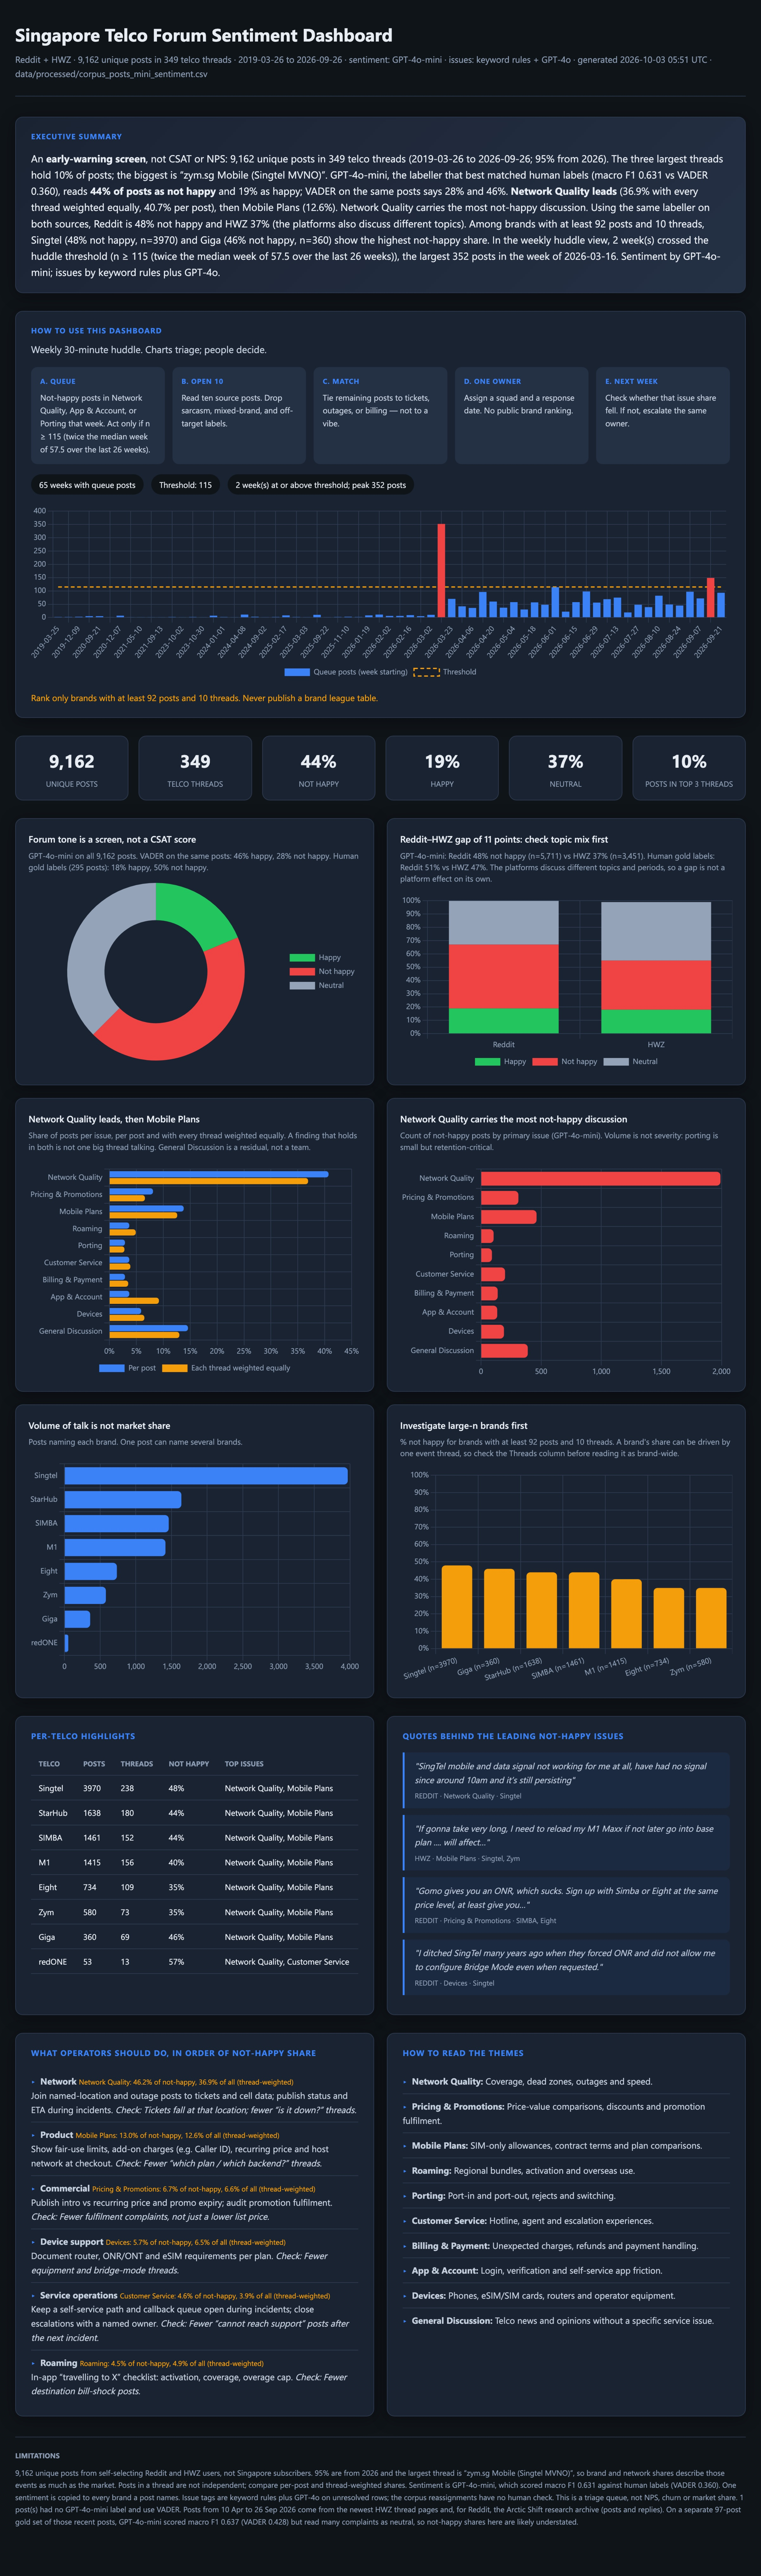
\includegraphics[width=0.9\textwidth,trim=0 2788 0 0,clip]{dashboard.pdf}
\caption{Dashboard, part 1 of 3: executive summary, weekly huddle playbook with the weekly queue chart and threshold, and headline counts.}
\label{fig:dash1}
\end{figure}

\begin{figure}[htbp]
\centering
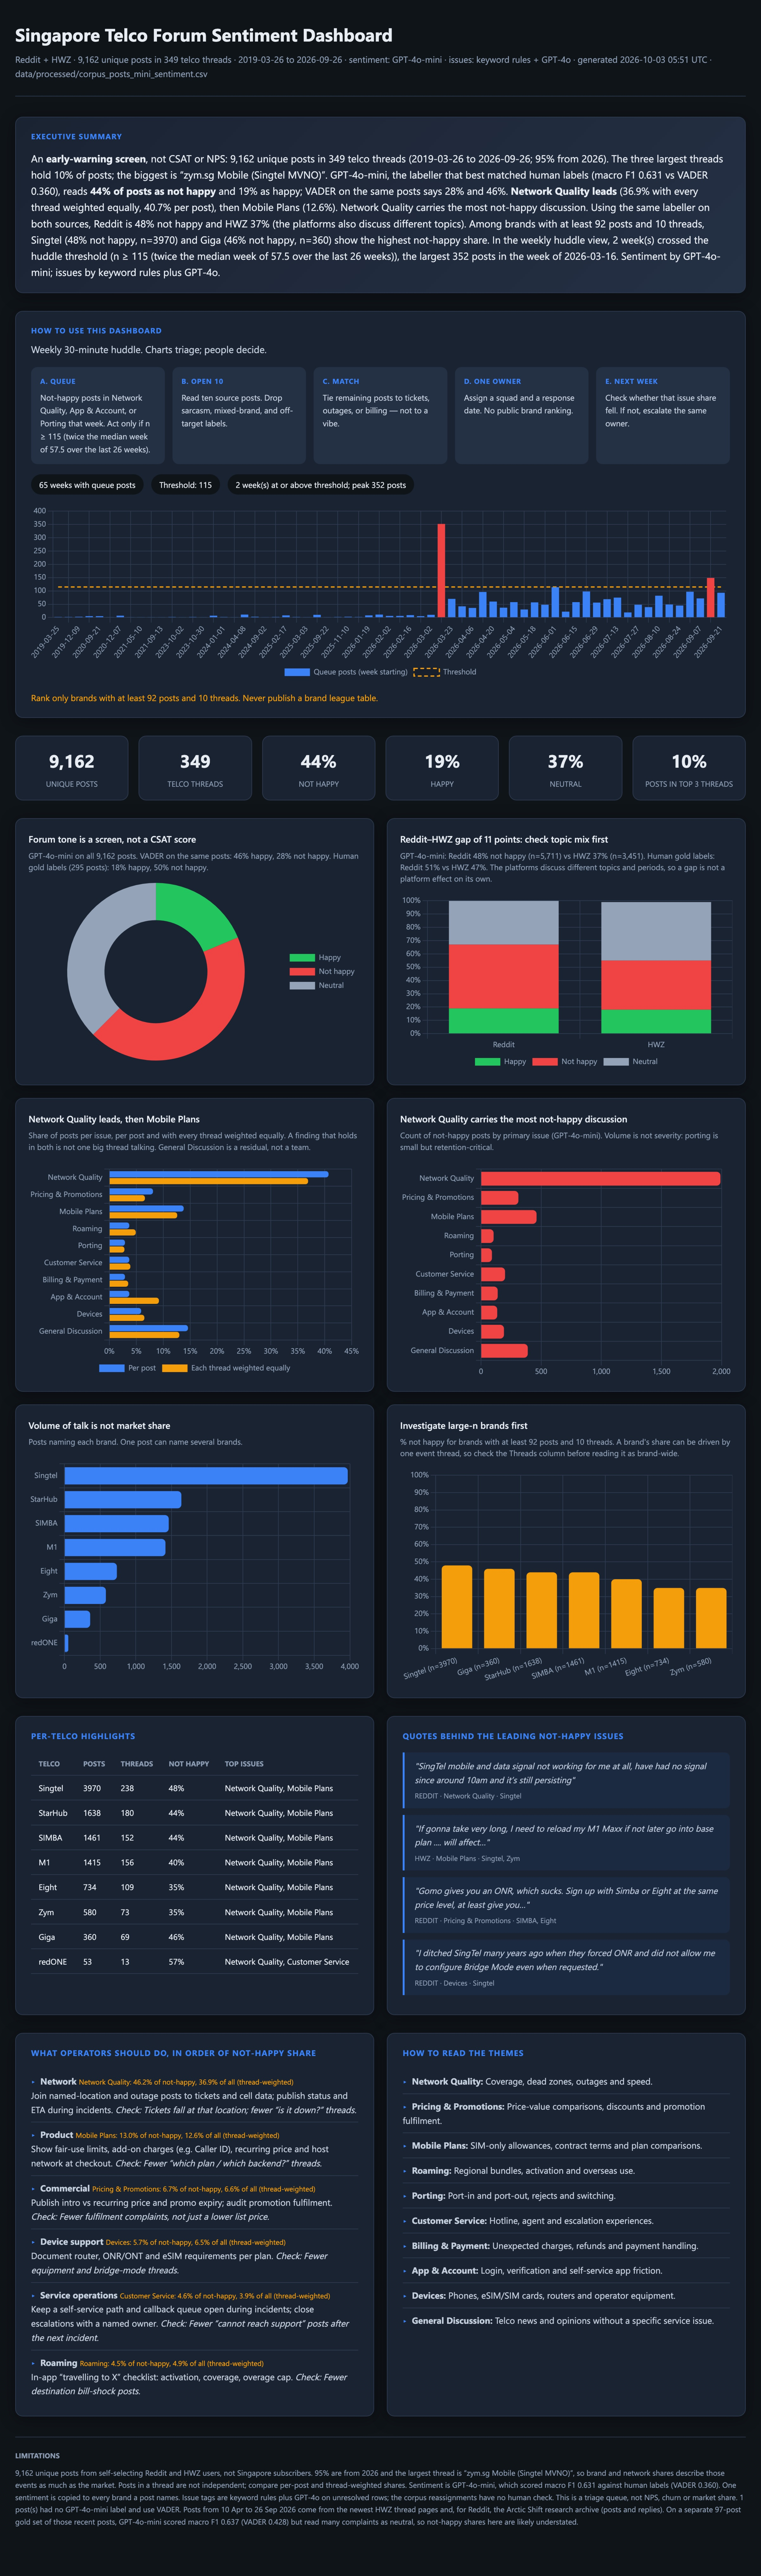
\includegraphics[width=0.9\textwidth,trim=0 1370 0 1272,clip]{dashboard.pdf}
\caption{Dashboard, part 2 of 3: overall tone, Reddit against HWZ, issue volume per post and thread-weighted, not-happy count by issue, brand volume and brand not-happy share.}
\label{fig:dash2}
\end{figure}

\begin{figure}[htbp]
\centering
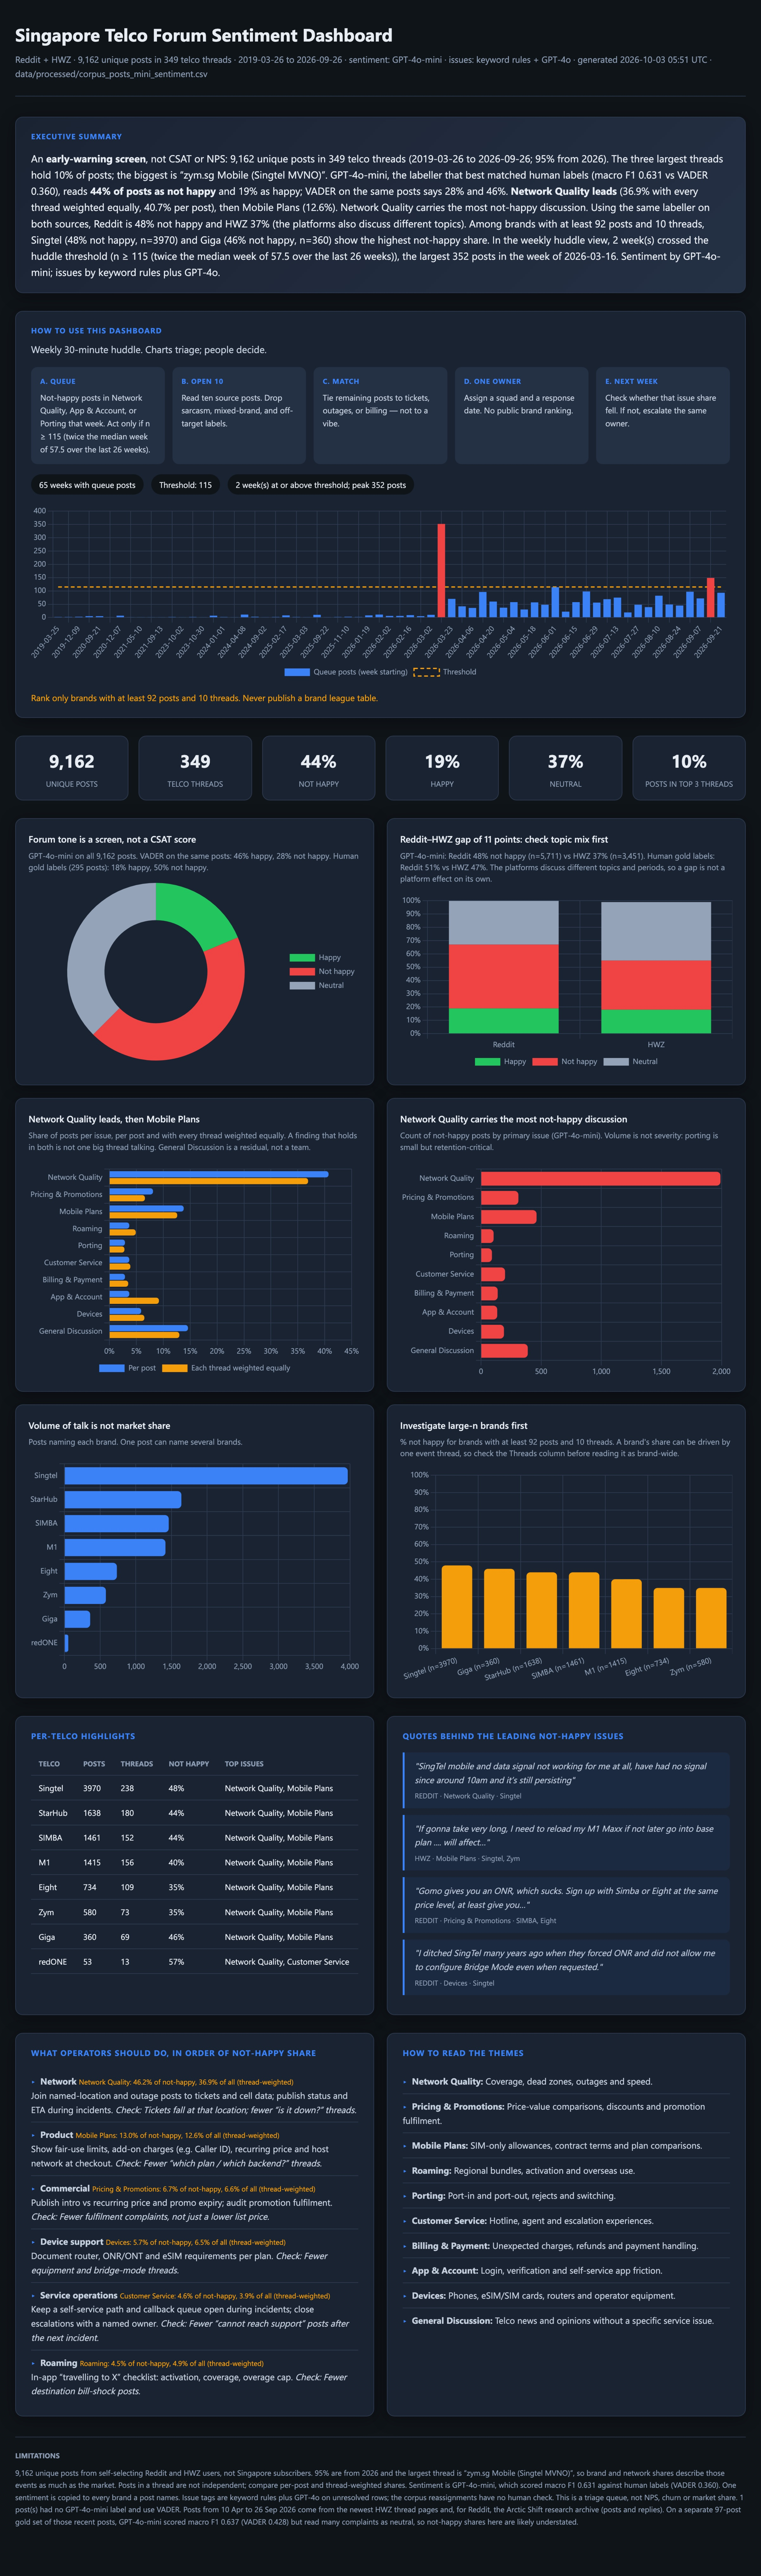
\includegraphics[width=0.9\textwidth,trim=0 13 0 2690,clip]{dashboard.pdf}
\caption{Dashboard, part 3 of 3: per-telco highlights, anonymised example posts for the leading not-happy issues, recommendations in order of not-happy share, and limitations.}
\label{fig:dash3}
\end{figure}

\section{Business Recommendations}

Each recommendation names an owner, an action and a check. They are ordered by each issue's share of not-happy discussion in the corpus. Forum counts are a triage queue, not proof of market failure.

\subsection{Network: communicate during incidents, then prove local fixes}

Network quality carries 46\% of not-happy discussion. Of 1,991 not-happy network posts, 621 sit in outage threads, and the huddle flagged both the March outage and the September StarHub broadband disruption. The first action is incident communication: a status page and proactive updates with an estimated restoration time, posted where customers are already asking. Outside outages, 289 not-happy network posts name a place such as MRT tunnels, homes or offices; network teams should join those posts to tickets and cell data. Success is a shorter time to the first public update during an incident, and fewer tickets at a named location after remediation.

\subsection{Product and commercial: make plan terms comparable}

Mobile plans (13\% of posts, in 202 threads) and pricing (8\%, 42\% not happy) are the second and third sources of not-happy discussion. Posts centre on terms customers discover late: fair-use limits on ``unlimited'' plans, add-on charges such as Caller ID (which posts note the three network operators charge for while SIMBA includes it), introductory prices that later change, and which host network an MVNO uses. Product and commercial teams should show fair-use rules, add-on charges, recurring price and host network at checkout. Success is fewer ``which plan?'' and hidden-charge threads.

\subsection{Devices and digital: fix equipment and app friction}

Device posts (6\%) cover eSIM failures and ONR/bridge-mode router policy; device support should publish router and eSIM requirements per plan. App and account problems are small per post but spread across 115 threads, including OTP failures on the SIMBA app in the September spike week; digital teams should watch forum posts after each app release. Success is fewer equipment threads and fewer ``cannot log in'' posts after a release.

\subsection{Customer service and billing: plan the incident aftercare}

Customer service (59\% not happy) and billing (53\%) are small but the most negative themes, and in the outage case study they were largely aftercare. Service and billing teams should publish the compensation rule with the incident notice and keep a self-service path open during outages. Success is fewer compensation and ``cannot reach support'' posts after the next incident.

\subsection{Lower-volume themes: roaming and porting}

Roaming (4\%) and porting (3\%) are small and mostly questions (31\% and 35\% not happy), so a ``travelling to X'' checklist and clearer port timelines are low-cost fixes rather than priorities.

\subsection{Insight huddle: operate the dashboard as an alert-and-review tool}

Do not publish a brand league table. A weekly 30-minute process is enough:

\begin{enumerate}
  \item flag not-happy posts in Network, App \& Account or Porting only when that week's volume clears a threshold set relative to a normal week (twice the recent median);
  \item open about ten source records and discard sarcasm, mixed-brand and off-target labels;
  \item triangulate with tickets, outages and billing;
  \item assign one owner and a response date;
  \item next week, check whether that issue's share fell.
\end{enumerate}

Use GPT-4o-mini for sentiment on the whole feed: labelling all 9,162 posts cost about \$0.28, so a daily run costs cents. For issues, keep keyword rules and apply GPT-4o to \texttt{general\_discussion} rows. On hard posts, GPT-4o labelling every post is more accurate and, at about \$0.0005 per post, affordable on a deduplicated feed. Keep a person in the loop before any public reply. That mix is the business reading of the evaluation, not a model contest.

\section{Limitations and Ethical Considerations}

\subsection{Representativeness and platform bias}

Forum contributors are self-selecting and are not Singapore mobile users at large. Findings use a corpus of 9,162 unique posts, after removing repeated copies (24,690 raw rows held 11,643 unique posts) and 96 off-topic threads. The corpus is 62\% Reddit, and 95\% of posts are from 2026; the few older posts are opening pages of long HWZ threads. Twelve per cent of posts sit in outage threads. Two collection artefacts are worth stating. Early HWZ scrapes read only the first page of each thread because of a page-counting bug; later scrapes add the newest pages. Reddit posts after 9~April~2026 come from the Arctic Shift research archive rather than Reddit directly, because Reddit blocks unauthenticated access and gates new API applications; the archive can miss content deleted before capture, and it includes replies that the earlier Reddit scraper skipped. There are no app-store reviews, tickets or NPS in the analysed set, so results cannot be generalised to market share, population sentiment, churn or Net Promoter Score.

\subsection{Unequal and dependent observations}

One record can mention several brands, so mention counts are not unique customers. Comments in a thread are not independent: they respond to a shared outage or launch. The report therefore shows thread-weighted shares beside per-post shares, and brand shares outside outage threads. Mixed-brand posts were often labelled \texttt{neutral}, which can hide a Singtel complaint sitting next to StarHub praise.

\subsection{Label quality and LLM misclassification}

The largest limit is the benchmark itself. It is one annotator, and two humans agree only fairly on typical posts ($\kappa=0.39$) and on small issue labels (Customer Service 0.28, Devices 0.16), mostly because the guide did not say whether a bare failure report is \texttt{not\_happy} or \texttt{neutral} (Section~\ref{sec:agreement}). Annotator~A treats such reports as complaints, and the guide now does too, but Annotator~A's labels have not yet been re-checked under that rule, so every score below carries that uncertainty, per-class scores for not happy and neutral most of all. Against this benchmark, GPT-4o-mini matches Annotator~A on about two-thirds of posts (accuracy 0.66, macro F1 0.641), and neutral is its weakest class (F1 0.57). One of 9,162 posts could not be labelled by GPT-4o-mini and falls back to VADER; 40 posts that failed in batches of ten were relabelled one at a time. All-post LLMs under-label Devices relative to rules (GPT-4o recall 0.24 versus 0.81 on the representative set, 0.33 versus 0.75 on the challenge set) and often return one topic when the post has several. Keyword rules over-trigger on generic terms such as ``plan''. Issue tagging is the weakest part of the system: the hybrid's 0.639 was measured on a set that includes the posts used to choose it, its gain over rules was not significant on held-out hard posts, and Customer Service scores below 0.55 for every method. The corpus issue reassignments have no second human check. These errors are prompt- and snapshot-specific. Forum text sent to a vendor API is also a privacy limit: production jobs must not submit NRIC, phone numbers or other identifiers. The defensible stance is triage plus human review, not automated league tables.

\subsection{Privacy and responsible use}

Although forum posts are publicly accessible, public availability does not remove ethical obligations. Reports should avoid usernames and unnecessary verbatim quotations, minimise stored identifiers, restrict raw-data access and comply with platform terms. The system should analyse themes, not profile individuals. Credentials and API keys must be stored in environment variables or a secret manager and must never appear in code, reports or version control.

\section{Future Work}
\label{sec:future}

\begin{enumerate}
  \item Raise human agreement first, because every other score is measured against these labels. Adjudicate the A--B disagreements in a separate file, relabel Annotator~A's overlap rows under the failure-report rule, and have the second annotator label more posts, especially Customer Service, Devices and App \& Account, where issue agreement is lowest ($\kappa$ 0.16 to 0.28). Then recompute $\kappa$ for sentiment and for each issue label. Until the labels are stable, a change in issue F1 cannot be told apart from annotation noise.
  \item Improve issue tagging once the labels are stable. It is the weakest result (hybrid macro F1 0.639 on typical posts, 0.509 on held-out hard posts), and Customer Service is the weakest label (F1 0.42 to 0.53 across methods). Add support-journey terms to the rules (agent, live chat, ticket, escalate, ``backend team''), give the GPT-4o pass a few labelled examples for each weak label, and score the change on held-out posts before adopting it.
  \item Compare the hybrid with GPT-4o labelling every post on a fresh held-out sample, since the two gold sets disagree on which is better.
  \item Spot-check the corpus rows that GPT-4o moved out of \texttt{general\_discussion}, especially the extra network-quality tags, before treating huddle counts as incidents.
  \item Add target-aware sentiment, so that a post praising one operator and criticising another yields a label per brand.
  \item Validate dashboard alerts against internal service tickets and network events before operational deployment.
\end{enumerate}

\section{Conclusion}

This project demonstrates a complete technical path from online forum collection to operator action. On 9,162 unique posts across six months, network quality dominates both the volume and the negativity of discussion, followed by plan terms and pricing. About two in five posts are not happy under every weighting; Reddit and HWZ differ mainly in topic rather than tone, and no brand stands out beyond small, weighting-sensitive differences, with Eight consistently the least negative. The March 2026 Singtel outage shows why this matters: 45 outage threads hold 12\% of posts but are 71\% not happy, and they made Singtel and Reddit look more negative than they are. The weekly huddle view flagged that outage and a later multi-brand bad week, and nothing else.

The analysis also shows why model governance matters. On 392 blinded human labels covering the whole collection period, gpt-4o-mini-2024-07-18 raises sentiment macro F1 from 0.380 (VADER) to 0.641; the gain holds on hard posts (0.773 versus 0.491), gpt-4o-2024-08-06 adds nothing for sentiment at about 17 times the cost, and repeated runs are stable. Two human annotators agree only fairly, but almost entirely over one ambiguous rule, and the model agrees with each of them about as well as they agree with each other. For issues the evidence is split: rules plus GPT-4o on unresolved posts is best on typical posts (0.639), and GPT-4o labelling every post is best on hard ones (0.596). The defensible deployment is LLM sentiment, rules plus a targeted LLM pass for issues, and human review of alerts, as an early-warning layer alongside, rather than in place of, customer-service and network data.

\begin{thebibliography}{9}

\bibitem{arcticshift}
A.~Heitmann,
``Arctic Shift: Reddit data archive and download tools,''
GitHub repository, \url{https://github.com/ArthurHeitmann/arctic_shift}, accessed 2026.

\bibitem{pang2008opinion}
B.~Pang and L.~Lee,
``Opinion Mining and Sentiment Analysis,''
\textit{Foundations and Trends in Information Retrieval}, vol.~2, no.~1--2, pp.~1--135, 2008.

\bibitem{liu2012sentiment}
B.~Liu,
\textit{Sentiment Analysis and Opinion Mining},
Synthesis Lectures on Human Language Technologies, Morgan \& Claypool, 2012.

\bibitem{hutto2014vader}
C.~J. Hutto and E.~Gilbert,
``VADER: A Parsimonious Rule-based Model for Sentiment Analysis of Social Media Text,''
\textit{Proceedings of the Eighth International AAAI Conference on Weblogs and Social Media},
pp.~216--225, 2014.

\bibitem{openai2024gpt4o}
OpenAI,
``GPT-4o System Card,''
arXiv:2410.21276, 2024.

\bibitem{landis1977kappa}
J.~R. Landis and G.~G. Koch,
``The Measurement of Observer Agreement for Categorical Data,''
\textit{Biometrics}, vol.~33, no.~1, pp.~159--174, 1977.

\bibitem{cohen1960kappa}
J.~Cohen,
``A Coefficient of Agreement for Nominal Scales,''
\textit{Educational and Psychological Measurement}, vol.~20, no.~1, pp.~37--46, 1960.

\bibitem{efron1993bootstrap}
B.~Efron and R.~J. Tibshirani,
\textit{An Introduction to the Bootstrap},
Chapman \& Hall, 1993.

\end{thebibliography}

\appendix
\section{Repository-to-Report Traceability}

\begin{longtable}{@{}p{0.33\textwidth}p{0.61\textwidth}@{}}
\toprule
\textbf{Repository artifact} & \textbf{Evidence used in this report} \\
\midrule
\endfirsthead
\toprule
\textbf{Repository artifact} & \textbf{Evidence used in this report} \\
\midrule
\endhead
\texttt{README.md} & Pipeline scope, command sequence, script responsibilities and default models \\
\texttt{Project\_\allowbreak{}Progress.md} & Data inventory, stated milestones, dashboard findings and planned evaluation work \\
\texttt{processing/\allowbreak{}preprocess.py} & Normalisation and filtering design \\
\texttt{processing/\allowbreak{}telco\_\allowbreak{}labeler.py} & Brand matching, VADER thresholds and optional GPT-4o-mini sentiment \\
\texttt{processing/\allowbreak{}issue\_\allowbreak{}extraction.py} & Taxonomy, keyword rules and batched GPT-4o unresolved hybrid \\
\texttt{models/\allowbreak{}llm\_\allowbreak{}evaluation.py} & Blind comparison of VADER, keyword rules, GPT-4o-mini and GPT-4o \\
\texttt{llm\_\allowbreak{}comparison\_\allowbreak{}representative/\allowbreak{}metrics.json} & Mini $n=295$ confusion matrices, per-class P/R/F1, tokens, runtime and cost \\
\texttt{llm\_\allowbreak{}comparison\_\allowbreak{}representative\_\allowbreak{}gpt4o/\allowbreak{}metrics.json} & GPT-4o $n=295$ metrics, tokens, runtime and cost \\
\texttt{llm\_\allowbreak{}comparison\_\allowbreak{}representative\_\allowbreak{}gpt4o\_\allowbreak{}hybrid/\allowbreak{}metrics.json} & Unresolved-only hybrid scored on the same gold labels \\
\texttt{llm\_\allowbreak{}comparison\_\allowbreak{}challenge/\allowbreak{}metrics.json} & Separate $n=100$ hard-case mini metrics \\
\texttt{llm\_\allowbreak{}comparison\_\allowbreak{}challenge\_\allowbreak{}gpt4o/\allowbreak{}} and \texttt{\_\allowbreak{}hybrid/\allowbreak{}} & GPT-4o and hybrid on the held-out challenge set \\
\texttt{llm\_\allowbreak{}comparison\_\allowbreak{}representative\_\allowbreak{}rerun/\allowbreak{}} & Second GPT-4o-mini run for stability \\
\texttt{robustness\_\allowbreak{}summary.json} & Bootstrap intervals, stability, $\kappa$ per set, corpus outage and brand checks \\
\texttt{processing/\allowbreak{}build\_\allowbreak{}clean\_\allowbreak{}corpus.py}, \texttt{corpus\_\allowbreak{}summary.json} & Deduplication, off-topic thread filter, per-thread shares \\
\texttt{models/\allowbreak{}corpus\_\allowbreak{}llm\_\allowbreak{}sentiment.py}, \texttt{corpus\_\allowbreak{}posts\_\allowbreak{}mini\_\allowbreak{}sentiment\_\allowbreak{}summary.json} & Corpus GPT-4o-mini sentiment, tokens and cost \\
\texttt{qualitative\_\allowbreak{}disagreements.csv} & Rows where methods disagree with human labels \\
\texttt{issues\_\allowbreak{}summary.json} & Keyword-only full-corpus issue-label counts \\
\texttt{issues\_\allowbreak{}summary\_\allowbreak{}gpt4o\_\allowbreak{}hybrid.json} & Hybrid full-corpus issue-label counts after GPT-4o on unresolved rows \\
\texttt{dashboard/\allowbreak{}generate\_\allowbreak{}dashboard.py} & Dashboard (\texttt{index.html}): computed chart titles, weekly queue, recommendation order \\
\texttt{scrapers/\allowbreak{}reddit\_\allowbreak{}archive\_\allowbreak{}scraper.py}, \texttt{hwz\_\allowbreak{}forum\_\allowbreak{}scraper.py} & Collection from 10~April~2026 (Arctic Shift archive; HWZ newest pages) \\
\texttt{processing/\allowbreak{}prepare\_\allowbreak{}new\_\allowbreak{}posts.py} & Cleaning, labelling and issue rules for posts from 10~April, and merge into the full corpus \\
\texttt{processing/\allowbreak{}create\_\allowbreak{}recent\_\allowbreak{}gold\_\allowbreak{}set.py}, \texttt{recent\_\allowbreak{}sampling\_\allowbreak{}metadata.json} & Blind sample of 100 posts from 10~April, part of the representative set \\
\texttt{processing/\allowbreak{}build\_\allowbreak{}gold\_\allowbreak{}labels.py}, \texttt{gold\_\allowbreak{}labels.csv} & All gold sheets in one file \\
\texttt{models/\allowbreak{}score\_\allowbreak{}merged\_\allowbreak{}gold.py}, \texttt{merged\_\allowbreak{}gold\_\allowbreak{}scores.json} & Every method on the 392-post representative set; bootstrap intervals; model-vs-human $\kappa$ \\
\texttt{dashboard/\allowbreak{}Dash\_\allowbreak{}README.md} & Dashboard input row counts and generated summary \\
\bottomrule
\end{longtable}

\section{LLM Cost Breakdown}
\label{app:cost}

Table~\ref{tab:costbreakdown} splits every API job into input and output tokens and prices each side separately. Token counts are those returned by the API and saved in each job's metrics or checkpoint file. Prices are the list prices used at run time: \$0.15 and \$0.60 per million input and output tokens for GPT-4o-mini, and \$2.50 and \$10.00 for GPT-4o. The unresolved-issue pass ran in two parts (posts to 9~April and later posts), shown on separate rows and summed in Table~\ref{tab:cost}. The hybrid gold scores reuse GPT-4o predictions and added no cost, so they have no row. VADER and keyword rules make no API calls.

\begin{table}[H]
\centering
\footnotesize
\caption{LLM cost by job, split into input and output tokens}
\label{tab:costbreakdown}
\resizebox{\fitwidth}{!}{%
\begin{tabular}{llrrrrrr}
\toprule
\textbf{Job} & \textbf{Model} & \textbf{$n$} & \textbf{Input tokens} & \textbf{Output tokens} & \textbf{Input USD} & \textbf{Output USD} & \textbf{Total USD} \\
\midrule
Representative eval & GPT-4o-mini & 295 & 32,015 & 6,449 & 0.0048 & 0.0039 & 0.0087 \\
Challenge eval & GPT-4o-mini & 100 & 10,595 & 2,353 & 0.0016 & 0.0014 & 0.0030 \\
Representative rerun & GPT-4o-mini & 295 & 32,015 & 6,461 & 0.0048 & 0.0039 & 0.0087 \\
Representative eval & GPT-4o & 295 & 32,015 & 6,530 & 0.0800 & 0.0653 & 0.1453 \\
Challenge eval & GPT-4o & 100 & 10,595 & 2,325 & 0.0265 & 0.0232 & 0.0497 \\
Representative eval, later posts & GPT-4o & 93 & 10,079 & 2,062 & 0.0252 & 0.0206 & 0.0458 \\
Corpus unresolved issues, posts to 9 Apr & GPT-4o & 8,786 & 763,704 & 153,993 & 1.9093 & 1.5399 & 3.4492 \\
Corpus unresolved issues, later posts & GPT-4o & 3,711 & 288,965 & 62,556 & 0.7224 & 0.6256 & 1.3480 \\
Corpus sentiment, posts to 9 Apr & GPT-4o-mini & 1,711 & 167,071 & 37,552 & 0.0251 & 0.0225 & 0.0476 \\
Corpus sentiment, all posts & GPT-4o-mini & 9,162 & 937,564 & 237,275 & 0.1406 & 0.1424 & 0.2830 \\
\midrule
\textbf{Total} & & & 2,284,618 & 517,556 & 2.9403 & 2.4487 & \textbf{5.39} \\
\bottomrule
\end{tabular}%
}
\end{table}

Input tokens carry most of the token volume (about four to five times the output tokens in every job), but output tokens are priced four times higher, so each side contributes a similar share of the cost. Two jobs account for almost all of the spend: the GPT-4o issue pass on unresolved corpus rows (about \$4.80 of the total) and the GPT-4o-mini sentiment run on the full corpus (about \$0.28).

\section{Reproducibility}

Run every command from the repository root. \texttt{README.md} gives the full commands, flags and model settings. The main workflow runs in this order:

\begin{verbatim}
python scrapers/hwz_forum_scraper.py            # HWZ posts
python scrapers/reddit_archive_scraper.py       # Reddit posts (Arctic Shift)
python processing/preprocess.py
python processing/telco_labeler.py              # brand + VADER sentiment
python processing/issue_extraction.py           # keyword rules; --use-llm
                                                #   --llm-unresolved-only for GPT-4o
python processing/build_clean_corpus.py
python processing/prepare_new_posts.py          # posts from 10 April; --merge
python models/corpus_llm_sentiment.py           # GPT-4o-mini, clean corpus
python dashboard/generate_dashboard.py          # -> dashboard/index.html
python models/llm_evaluation.py                 # VADER/rules vs GPT-4o-mini, GPT-4o
python processing/build_gold_labels.py
python models/score_merged_gold.py              # no API calls
python models/robustness_checks.py              # no API calls
\end{verbatim}

The GPT-4o pass on unresolved rows and the corpus sentiment run have already been done and their outputs are saved, so they do not need to be repeated. Each run reads \texttt{OPENAI\_API\_KEY} from the environment. API credentials should be supplied through environment variables and excluded from all submitted material.


\end{document}
